\documentclass[a4paper»,8pt,french,fleqn]{report}
%Packages:

%Langages:
\usepackage[french]{babel}
\usepackage{lmodern}
\usepackage[T1]{fontenc}
\usepackage[utf8]{inputenc}

%AMS maths
\usepackage{amsmath, amssymb, amsfonts}

%Mise en page
\usepackage[top=2cm, right=2cm, bottom=2cm, left=2cm]{geometry}
\usepackage{fancyhdr}
\usepackage{enumerate}
\usepackage{color}
%Définition des macros
\usepackage{amsthm}

%Figures
\usepackage{tikz}
\usepackage{graphicx}
\usepackage{wrapfig}

%Symboles mathématiques
\usepackage{latexsym}
\usepackage{bm}

%Listings
\usepackage{listings}
\lstset{language=SQL}

%Titre et auteurs
\title{\textbf{SGBD - Projet Sport }\\\textit{Rapport du travail fourni}}

\author{PHILIPPI Alexande \& MAUPEU Xavier \& PAILLASSA Maxime}

\date{\today}

\begin{document}

\maketitle

\newpage

\tableofcontents

\newpage

\chapter*{Introduction}

Le projet consistait en la réalisation d'une base de données gérant les rencontres entre les clubs de basketball d'une fédération. Il fallait implémenter des requêtes permettant d'obtenir des informations sur les clubs, les équipes et les joueurs. Tel que les meilleurs joueurs, les classements des équipes au sein d'un club et/ou de la fédération. Afin d'intéragir avec la base et la faire évoluer simplement, des scripts d'insertion, de modification et de suppression devaient être implémentés via des formulaires python, java, php.

\chapter{Présentation du modèle}

\section{Schéma Entité-Association}

\begin{figure}[h]
  \centering
    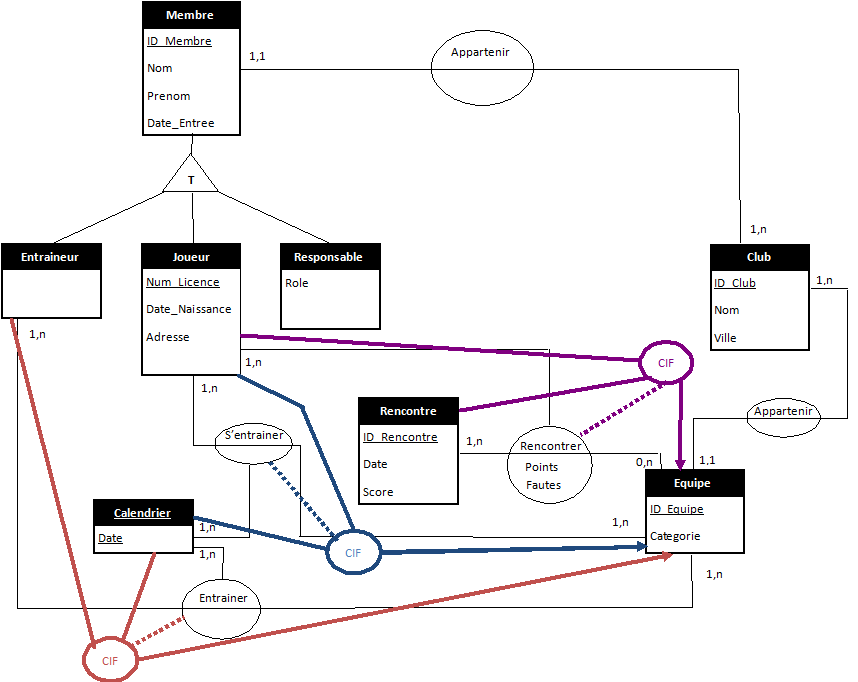
\includegraphics[scale=0.7]{Schema_EA.png}
    \label{fig:schema_ea}
    \caption{Schéma Entité-Association établi par l'équipe}
\end{figure}

D'après la figure \ref{fig:schema_ea}, plusieurs choix ont été fait dans la structuration de la base de données : \\

\begin{itemize}

\item Les joueurs n'appartiennent pas à une équipe mais à un club. Cela offre la possibilité de changer d'équipe un joueur à chaque rencontre. \\

\item Joueur, Responsable et Entraineur héritent de Membre. Par la contrainte de totalité un Membre doit être soit Joueur ou Responsable ou Entraineur, soit les trois à la fois, soit deux parmis les trois. \\

\item La contrainte d'intégrité fonctionnelle appliquée à Joueur et Rencontre permet d'associer un Joueur à une seule équipe lors d'une rencontre. De même pour les entrainements, à une date donnée, un entraineur entraîne une seule équipe et un joueur ne peut s'entraîner qu'avec une équipe.

\end{itemize}

\section{Schéma Relationnel}

On peut ensuite passer au schéma relationnel: \\
Club(\underline{ID\_Club}, Nom, Ville) \\ 
Membre(\underline{ID\_Membre}, #ID\_Club, Nom, Prenom, Date\_Entree) \\
Entraineur(\underline{#ID\_Membre}) \\
Joueur(\underline{Num\_Licence}, #ID\_Membre, Date\_Naissance, Adresse) \\ 
Responsable(\underline{#ID\_Membre}) \\
Rencontre (\underline{ID\_Rencontre}, Date\_Match) \\
Equipe(\underline{ID\_Equipe}, Categorie, #ID\_Club) \\
Rencontrer(\underline{#ID\_Membre}, \underline{ID\_Rencontre}, #ID\_Equipe, Points, Fautes) \\
Sentrainer(\underline{#ID\_Membre}, \underline{Date\_Entrainement}, #ID\_Equipe) \\
Entrainer(\underline{#ID\_Membre}, \underline{Date\_Entrainement}, #ID\_Equipe) 


\chapter{Implémentation}

L'interface entre l'utilisateur et la base de donnée a été faite en php. Les sous-parties suivantes présenteront les requêtes implémentées par onglet du site internet.

\section{Clubs}

Cette partie liste les différents clubs de la fédération avec pour renseignement : la ville, les responsables, le nombre d'équipes et le nombre de joueurs. Deux sous-requêtes sont implémentées dans \ref{club} afin d'obtenir le nombre d'équipes et de joueurs du club. 

\lstset{frame=single, caption={Requete information sur les clubs}, label=club}
\begin{lstlisting}

Select c.Nom, c.Ville, c.ID\_Club,
 (Select count(*) 
  From Equipe e
  Where c.ID\_club = e.ID\_Club) as NombreEquipe,

 (Select count(*) 
  From Joueur j, Membre m
  Where c.ID\_Club = m.ID\_Club
  and m.ID\_Membre = j.ID\_Membre) as NombreJoueur

From Club c;
\end{lstlisting}

\section{Equipes}

Dans l'onglet 'Equipes' il est possible de visualiser le classement des équipes de la fédération par catégorie. La catégorie est séléctionnée via un formulaire PHP et les résultats sont affichés dans un tableau HTML.

\lstset{frame=single, caption={Requête classement des équipes de la fédération par catégorie}, label=club}
\begin{lstlisting}

Select c.Nom,
  sum(e.Points > t.Points/2) as gagne,
  sum(e.Points = t.Points/2) as egual,
  sum(e.Points < t.Points/2) as perdu
  
From
  
  (Select ID\_Rencontre, e1.*,
    sum(r1.Points) as Points
  From Equipe e1, Rencontrer r1
  Where e1.ID\_Equipe = r1.ID\_Equipe
  Group by r1.ID\_Rencontre, e1.ID\_Equipe) e,

  (Select ID\_Rencontre,
    sum(r1.Points) as Points
  From Rencontrer r1
  Group by r1.ID\_Rencontre) t,
  
  Club c

Where e.ID\_Rencontre = t.ID\_Rencontre
  and e.ID\_Club = c.ID\_Club
  and e.Categorie = '\$\_POST['categorie']'
Group by e.ID\_Equipe
Order by gagne DESC, egual DESC, perdu DESC

\end{lstlisting}

Le classement peut-être restreint aux clubs sans distinction des catégories. La requête est sensiblement la même, si ce n'est que la catégorie n'apparait plus comme un critère de sélection et le nom du club devient le premier critère d'ordonnancement de la table (avant 'gagne', 'egual' et 'perdu'). 


\section{Joueurs}
Dans l'onglet 'Joueurs', les joueurs de la fédération sont classés par clubs avec des informations comme le nom, prénom, numéro de licence... La moyenne des points marqués et des fautes faites, ainsi que leur écart type sont calculés via les fonctions SQL ``avg'' et ``std''. La requête \ref{joueur} permet de collecter ces informations dans les tables de la base de données.

\lstset{frame=single, caption={Requête classement des joueurs par club}, label=joueur}
\begin{lstlisting}
Select c.Nom as Nom\_Club, j.ID\_Membre, j.Num\_Licence, m.Date\_Entree, m.Nom, m.Prenom, j.Adresse, j.Date\_Naissance,
  avg(r.Points) as MoyennePoints,
  std(r.Points) as EcartTypePoints,
  avg(r.Fautes) as MoyenneFautes,
  std(r.Fautes) as EcartTypeFautes

From Membre m, Joueur j, Rencontrer r, Rencontre a, Club c
Where m.ID\_Membre = j.ID\_Membre
  and r.ID\_Membre = m.ID\_Membre
  and a.ID\_Rencontre = r.ID\_Rencontre
  and Year(a.Date\_match) = Year(Now())
  and c.ID\_Club = m.ID\_Club
Group by c.Nom, j.ID\_Membre
\end{lstlisting}

La ligne '\textit{and Year(a.Date\_match) = Year(Now())}' permet de selectionner seulement les matchs se déroulant pendant la saison courante. Nous sommes partis du principe qu'une saison se déroulait du 1er Janvier d'une année au 31 Décembre de cette même année, pour simplifier les choses.


\section{Graphique}
Grace à l'utilisation de l'extension gd2 de PHP, il est possible de créer des graphiques. Pour chaque mois d'une année et un joueur sont tracés, les points gagnés, les fautes faites et le nombre de matchs gagnés et perdus. La figure \ref{fig:graph} est un exemple de graphique obtenu après application de la requête \ref{graphique}.

\lstset{frame=single, caption={Requête des statistiques pour un joueur}, label=graphique}
\begin{lstlisting}
Select Month(Date\_Match) AS mois,
  Sum(r.Points) as PointsMois,
  Sum(r.Fautes) as FautesMois,
  Sum(
    (Select sum(r1.Points)
    From Rencontrer r1
    Where r1.ID\_Rencontre = r.ID\_Rencontre
    and r1.ID\_Equipe = r.ID\_Equipe)
    >
    (Select sum(r1.Points)
    From Rencontrer r1
    Where r1.ID\_Rencontre = r.ID\_Rencontre)/2) as Gagne,
    
count(r.ID\_Rencontre) as NombreMatch

From Joueur j, Rencontrer r, Rencontre a
Where j.ID\_Membre = \$idJoueur
  and j.ID\_Membre = r.ID\_Membre
  and r.ID\_Rencontre = a.ID\_Rencontre
  and Year(Date\_Match) = \$annee
Group by mois 
Order by mois ASC
\end{lstlisting}

\begin{figure}[h]
  \centering
    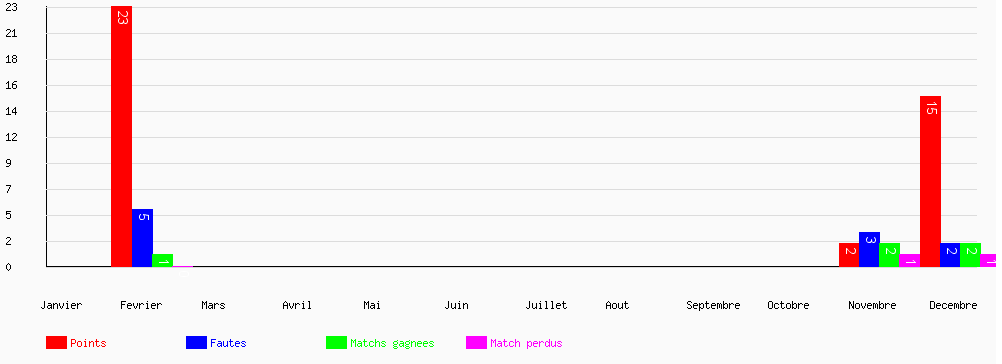
\includegraphics[scale=0.5]{graphe.png}
    \label{fig:graph}
    \caption{Graphique des matchs pour un joueur au cours de la saison 2014}
\end{figure}


\section{Matchs}

\lstset{frame=single, caption={Requête des matchs}, label=match}
\begin{lstlisting}
Select Distinct r.ID\_Equipe, c.Nom, e.Categorie, re.Date\_match, re.ID\_Rencontre,
  sum(r.Points) as points, 
  sum(r.Fautes) as fautes 

From Rencontre re, Rencontrer r, Equipe e, Club c

Where e.ID\_Equipe = r.ID\_Equipe
  and re.ID\_Rencontre = r.ID\_Rencontre
  and e.ID\_Club = c.ID\_Club

Group by e.ID\_Equipe, r.ID\_Rencontre
Order by re.Date\_match, re.ID\_Rencontre, points DESC');
\end{lstlisting}

Une autre variante de cette requête permet de sélectionner les matchs par date de rencontre.

\chapter*{Conclusion}

\end{document}
